\chapter{Configuration management}
A software is made of many parts (i.e.\@ documents, programs, etc.) with different instances (customer, platforms, etc.) and thousands of separate documents are generated for a large software system. A software system changes because of different instances of software for different customers and because the same software changes over time.

Therefore, it is needed to identify the history of a document (versioning), the correct set of documents for a specific need (configuration), who can access and change what (change control) and how the system is obtained (build). \emph{Configuration management} permits to identifiy and manage parts of software, control access and changes to parts and allow to rebuild previous version of software.

\section{Versioning}
\emph{Versioning} permits to keep track of versions using same names or different version names in such a way that a user decides when to change version (commit operation) and that is always possible to recover a past version.

\paragraph{Configuration item}
A configuration item (CI) is an element under configuration control. It is characterized by a name and a version number and all its version numbers are kept. The user decides to change version number with specific operation (\textbf{commit}) and it is possible to retrieve any version.

It is the basic unit for the configuration management system, e.g.\@ a work product or piece of software that is treated as a single entity for the purpose of configuration management. It may correspond to one or more documents or one or more programs.

Not all documents in a project become a configuration item. If all documents are considered configuration item, a large overhead is introduced but, on the other hand, if no documents are considered configuration item, no history is available and there is no information on configurations.

\paragraph{Configuration}
Configuration items have depencencies among them, some a re syntactically defined (e.g.\@ \texttt{\#include} or \texttt{import} statements) but most are not such as requirement and test cases. This requires a way to treat sets of configuration items, i.e.\@ \emph{traceability}.

\begin{figure}[hbtp]
\centering
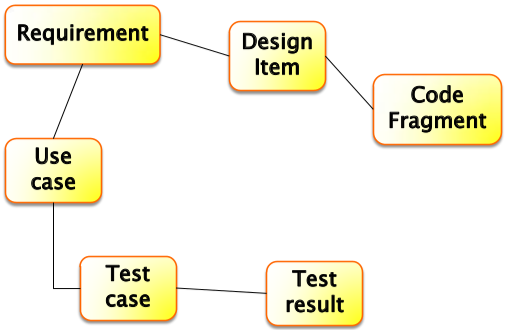
\includegraphics[scale=0.3]{images/dependency_traceability.png}
\caption{Dependency and traceability}
\end{figure}

A configuration is defined as a set of items, each in a specific version and, generally, it includes not only source code. The same configuration item may appear in different configuration. Therefore, also configuration has version. There are two main approaches to identify a configuration:
\begin{enumerate}
\item ID for configuration, ID for configuration item: CVS;
\item ID for configuration, same ID for all configuration items in the configuration: Subversion, Git.
\end{enumerate}

\subparagraph{Approach 1}
Configuration items numbering and configuration numbering are independent. In this way, it is clear when a configuration item changes but the name of configuration item and configuration are managed separately.

\begin{figure}[hbtp]
\centering
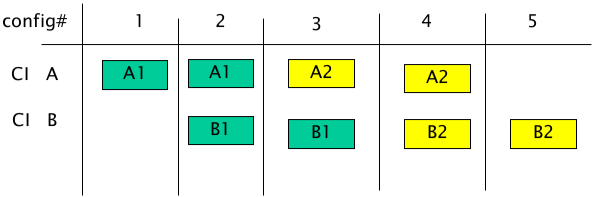
\includegraphics[scale=0.3]{images/configuration_approach1.png}
\caption{Configuration - Approach 1}
\end{figure}

\subparagraph{Approach 2}
Configuration number changes on every change. Items inherits the configuration numbering. In this way, configuration items and configuration are managed together, therefore it is unclear when a configuration item changes.

\begin{figure}[hbtp]
\centering
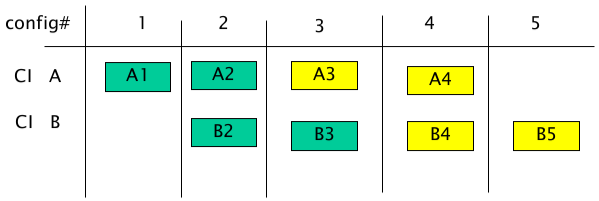
\includegraphics[scale=0.3]{images/configuration_approach2.png}
\caption{Configuration - Approach 2}
\end{figure}

\paragraph{Version}
A version is a particular instance of a configuration item at a certain point in time. Each instance as a unique number and each configuration has a unique number.

\paragraph{Baseline}
A baseline identifies a configuration in a stable, frozen form. Not all configurations are baselines.

\section{Change control}
Typically, a team develops a software. Hence, many people need to access parts of software contained in a common repository (shared folder) in such a way that all can read and write documents and programs.

\begin{description}
\item [Repository] Place where configuration items and configurations are stored.
\item [Workspace] Place where users work, on copies of configuration items.
\end{description}

\begin{figure}[hbtp]
\centering
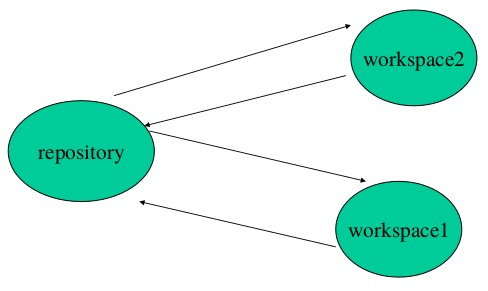
\includegraphics[scale=0.3]{images/repository_workspace.png}
\end{figure}

\subsection{Repository}
It can implemented as a shared folder, containing shared files, on file server or using a CMS\footnote{Content Management System} tool with change control (check-in, check-out). Changes must be disciplined, it requires knowledge about who controls, what is controlled and how control is implemented.

A repository can be implemented exploiting different approaches:
\begin{itemize}
\item Local: repository and user on the same machine;
\item Centralized: repository on a single server, many users (clients) can access and obtain copies of files;
\item Distributed: repository mirrored on all servers/clients.
\end{itemize}

\begin{description}
\item [Check-out] Extraction of configuration items from repository with purpose of changing it or not. After checkout. next users are notified.
\item [Check-in] Insertion of configuration items under control.
\end{description}

\begin{center}
\begin{tabularx}{\textwidth}{X|X}
Check in/out & File system \\ 
\hline 
Confiuration items are in repository & Files are in shared directory \\ 
\hline 
To read/write a configuration item, user needs to perform checkout & Any user can get copy of file, or work on original \\
\hline 
After checkout, next user knows that configuration item is used by someone else & Users can work on copies of file without knowing that others are doing the same
\end{tabularx} 
\end{center}

\paragraph{Scenarios}
\subparagraph{Lock modify unlock - Serialization}
One can change at a time. Thus, no parallel work and delays. Problems if locker forgets to unlock. As shown in figure~\ref{img:lock_modify_unlock}, first check out locks the file and no other checkouts are allowed until checkin.

\begin{figure}[hbtp]
\centering
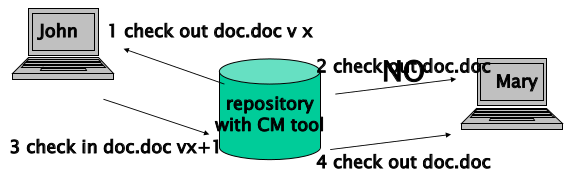
\includegraphics[scale=0.5]{images/lock_modify_unlock.png}
\caption{Lock modify unlock}
\label{img:lock_modify_unlock}
\end{figure}

\subparagraph{Copy modify merge}
Many change in parallel, the merge. It is more flexible but requires care to resolve the conflict. As shown in figure~\ref{img:copy_modify_merge}, the second check in signals conflict. User has to do manual merge of \emph{x+1} and \emph{x+1'} in \emph{x+2}.

\begin{figure}[hbtp]
\centering
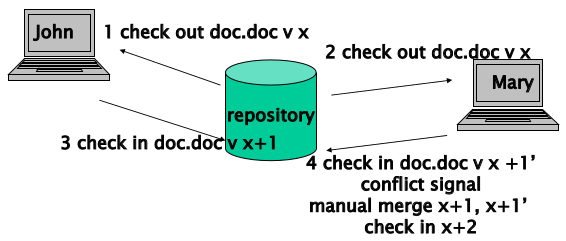
\includegraphics[scale=0.5]{images/copy_modify_merge.png}
\caption{Copy modify merge}
\label{img:copy_modify_merge}
\end{figure}

\paragraph{CMS approaches}
\begin{itemize}
\item Local: RCS;
\item Centralized: CSV, Subversion;
\item Distributed: Git, Mercurial, Bazaar.
\end{itemize}

Very often, it is needed to proceed with \emph{parallel versions}, while keeping trace of common origin, as shown in figure~\ref{img:branches_merges}. For example, when some developers work on branch to fix defect, while other work to add functionalities.

\begin{figure}[hbtp]
\centering
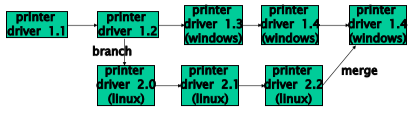
\includegraphics[scale=0.5]{images/branches_merges.png}
\caption{Copy modify merge}
\label{img:branches_merges}
\end{figure}

\paragraph{CM Planning}
\emph{CM plan} contains key CM related choices and policies in a project, i.e.\@ requirement and design documents, source files, test plan, test cases, configuration files, parameters, tools used in the production chain. It is needed to define which CM tool to use, what should and should not be a configuration item, control policies and who is the CM manager.

\paragraph{Build}
System building is the process of compiling and linking software components into an executable system. Different systems are built from different combinations of components.

Systems are normally represented for building by specifying the filename to be processed by building tools. Dependencies between these are described to the building tools (e.g.\@ Make, Ant, Maven). Mistakes can be made as users lose track of which objects are stored in which files. A system modelling language addresses this problem by using a logical rather than a physical system representation.

\begin{figure}[hbtp]
\centering
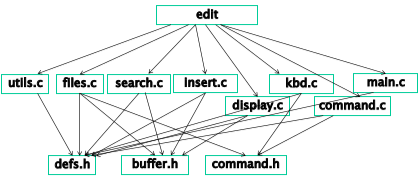
\includegraphics[scale=0.5]{images/dependencies.png}
\caption{Example of dependencies}
\end{figure}